% Options for packages loaded elsewhere
\PassOptionsToPackage{unicode}{hyperref}
\PassOptionsToPackage{hyphens}{url}
\PassOptionsToPackage{dvipsnames,svgnames,x11names}{xcolor}
%
\documentclass[
  super,
  review,
  3p]{elsarticle}

\usepackage{amsmath,amssymb}
\usepackage{iftex}
\ifPDFTeX
  \usepackage[T1]{fontenc}
  \usepackage[utf8]{inputenc}
  \usepackage{textcomp} % provide euro and other symbols
\else % if luatex or xetex
  \usepackage{unicode-math}
  \defaultfontfeatures{Scale=MatchLowercase}
  \defaultfontfeatures[\rmfamily]{Ligatures=TeX,Scale=1}
\fi
\usepackage{lmodern}
\ifPDFTeX\else  
    % xetex/luatex font selection
\fi
% Use upquote if available, for straight quotes in verbatim environments
\IfFileExists{upquote.sty}{\usepackage{upquote}}{}
\IfFileExists{microtype.sty}{% use microtype if available
  \usepackage[]{microtype}
  \UseMicrotypeSet[protrusion]{basicmath} % disable protrusion for tt fonts
}{}
\makeatletter
\@ifundefined{KOMAClassName}{% if non-KOMA class
  \IfFileExists{parskip.sty}{%
    \usepackage{parskip}
  }{% else
    \setlength{\parindent}{0pt}
    \setlength{\parskip}{6pt plus 2pt minus 1pt}}
}{% if KOMA class
  \KOMAoptions{parskip=half}}
\makeatother
\usepackage{xcolor}
\setlength{\emergencystretch}{3em} % prevent overfull lines
\setcounter{secnumdepth}{5}
% Make \paragraph and \subparagraph free-standing
\ifx\paragraph\undefined\else
  \let\oldparagraph\paragraph
  \renewcommand{\paragraph}[1]{\oldparagraph{#1}\mbox{}}
\fi
\ifx\subparagraph\undefined\else
  \let\oldsubparagraph\subparagraph
  \renewcommand{\subparagraph}[1]{\oldsubparagraph{#1}\mbox{}}
\fi


\providecommand{\tightlist}{%
  \setlength{\itemsep}{0pt}\setlength{\parskip}{0pt}}\usepackage{longtable,booktabs,array}
\usepackage{calc} % for calculating minipage widths
% Correct order of tables after \paragraph or \subparagraph
\usepackage{etoolbox}
\makeatletter
\patchcmd\longtable{\par}{\if@noskipsec\mbox{}\fi\par}{}{}
\makeatother
% Allow footnotes in longtable head/foot
\IfFileExists{footnotehyper.sty}{\usepackage{footnotehyper}}{\usepackage{footnote}}
\makesavenoteenv{longtable}
\usepackage{graphicx}
\makeatletter
\def\maxwidth{\ifdim\Gin@nat@width>\linewidth\linewidth\else\Gin@nat@width\fi}
\def\maxheight{\ifdim\Gin@nat@height>\textheight\textheight\else\Gin@nat@height\fi}
\makeatother
% Scale images if necessary, so that they will not overflow the page
% margins by default, and it is still possible to overwrite the defaults
% using explicit options in \includegraphics[width, height, ...]{}
\setkeys{Gin}{width=\maxwidth,height=\maxheight,keepaspectratio}
% Set default figure placement to htbp
\makeatletter
\def\fps@figure{htbp}
\makeatother

\usepackage{lineno}\linenumbers
\date{2024-04-15}
\makeatletter
\@ifpackageloaded{caption}{}{\usepackage{caption}}
\AtBeginDocument{%
\ifdefined\contentsname
  \renewcommand*\contentsname{Table of contents}
\else
  \newcommand\contentsname{Table of contents}
\fi
\ifdefined\listfigurename
  \renewcommand*\listfigurename{List of Figures}
\else
  \newcommand\listfigurename{List of Figures}
\fi
\ifdefined\listtablename
  \renewcommand*\listtablename{List of Tables}
\else
  \newcommand\listtablename{List of Tables}
\fi
\ifdefined\figurename
  \renewcommand*\figurename{Figure}
\else
  \newcommand\figurename{Figure}
\fi
\ifdefined\tablename
  \renewcommand*\tablename{Table}
\else
  \newcommand\tablename{Table}
\fi
}
\@ifpackageloaded{float}{}{\usepackage{float}}
\floatstyle{ruled}
\@ifundefined{c@chapter}{\newfloat{codelisting}{h}{lop}}{\newfloat{codelisting}{h}{lop}[chapter]}
\floatname{codelisting}{Listing}
\newcommand*\listoflistings{\listof{codelisting}{List of Listings}}
\makeatother
\makeatletter
\makeatother
\makeatletter
\@ifpackageloaded{caption}{}{\usepackage{caption}}
\@ifpackageloaded{subcaption}{}{\usepackage{subcaption}}
\makeatother
\journal{Dr. Farid}
\ifLuaTeX
  \usepackage{selnolig}  % disable illegal ligatures
\fi
\usepackage[]{natbib}
\bibliographystyle{elsarticle-num}
\nocite{*}
\usepackage{bookmark}

\IfFileExists{xurl.sty}{\usepackage{xurl}}{} % add URL line breaks if available
\urlstyle{same} % disable monospaced font for URLs
\hypersetup{
  pdftitle={Beyond Trial and Error: A Machine Learning Approach to Optimal Centrifugal Pump Impeller Trimming},
  pdfauthor={Mohamed Farid Khalil; Mohammed Twheed Khater; Seif Ibrahim Hassan},
  pdfkeywords={Pump impeller trimming, Neural networks, Hyperparameter
optimization, Genetic algorithms, Mean squared error},
  colorlinks=true,
  linkcolor={blue},
  filecolor={Maroon},
  citecolor={Blue},
  urlcolor={Blue},
  pdfcreator={LaTeX via pandoc}}

\setlength{\parindent}{6pt}
\begin{document}

\begin{frontmatter}
\title{Beyond Trial and Error: A Machine Learning Approach to Optimal
Centrifugal Pump Impeller Trimming \\\large{A Genetic Algorithm
Hyperparameter Optimization Approach} }
\author[1]{Mohamed Farid Khalil%
\corref{cor1}%
\fnref{fn1}}
 \ead{mfaridkhalil@yahoo.com} 
\author[1]{Mohammed Twheed Khater%
%
\fnref{fn2}}
 \ead{mohammedtwheed@gmail.com} 
\author[1]{Seif Ibrahim Hassan%
%
\fnref{fn3}}


\affiliation[1]{organization={Alexandria University, Mechanical
Engineering},city={Alexandria},country={Egypt},countrysep={,},postcodesep={}}

\cortext[cor1]{Corresponding author}
\fntext[fn1]{Professor, Mechanical Engineering Department, Faculty of
Engineering, Alexandria University, Alexandria, Egypt.}
\fntext[fn2]{Undergraduate, Mechanical Engineering Department, Faculty
of Engineering, Alexandria University, Alexandria, Egypt.}
\fntext[fn3]{Undergraduate, Mechanical Engineering Department, Faculty
of Engineering, Alexandria University, Alexandria, Egypt.}
        
\begin{abstract}
This paper proposes a genetic algorithm (GA)-based methodology to
optimize hyperparameters for artificial neural networks (NNs) applied to
pump impeller trimming. Traditionally, impeller trimming relies on
expert knowledge and empirical methods, leading to time-consuming and
potentially suboptimal outcomes. This work introduces a data-driven
approach using NNs trained to predict the impeller diameter (D) and pump
power (P), which can be calculated from flow rate (Q), density
(\(\rho\)), head (H), and efficiency (\(\eta\)) using the equation P =
(Q * \(\rho\) * g * H) / \(\eta\). based on the desired operating point
(flow rate (Q) and head (H)). A GA is employed to identify the optimal
NN hyperparameters, including hidden layer size, training function,
activation function, and maximum epochs. The goal is to minimize the
mean squared error (MSE) between the network's predictions and the
actual performance data. The paper details the implementation of the GA
optimization process and discusses the key components and their
significance in achieving optimal impeller trimming through NN
predictions.
\end{abstract}





\begin{keyword}
    Pump impeller trimming \sep Neural networks \sep Hyperparameter
optimization \sep Genetic algorithms \sep 
    Mean squared error
\end{keyword}
\end{frontmatter}
    
\begin{nomenclature}
\begin{deflist}[AA] %[AAAA] if you have 4 letters max for example
\defitem{NN}\defterm{Neural Network}
\defitem{GA}\defterm{Genetic Algorithm}

\end{deflist}

\begin{deflist}[AAA] %[AAAA] if you have 4 letters max for example
\defitem{MSE}\defterm{Mean Square Erorr}
\defitem{NNs}\defterm{Neural Networks}
\defitem{CNNs}\defterm{Convolution Neural Networks}
\defitem{RNNs}\defterm{Recurrent Neural Networks}

\end{deflist}
\end{nomenclature}

\section{Introduction}\label{introduction}

Pump impeller trimming is a crucial procedure in optimizing the
performance of centrifugal pumps for specific operating conditions. It
involves modifying the impeller geometry, typically by removing material
from the blades, to achieve desired hydraulic characteristics such as
flow rate (Q), head (H), and efficiency (\(\eta\)). Traditionally, this
process has relied heavily on \textbf{empirical methods and engineering
expertise}. These methods can be time-consuming, require significant
trial-and-error experimentation, and may not always achieve the optimal
trimming configuration.

The introduction of artificial neural networks (NNs) offers a promising
\textbf{data-driven} alternative for automating and enhancing the pump
impeller trimming process. NNs excel at modeling complex relationships
between input data and desired outputs. By training an NN on a dataset
of impeller designs and their corresponding performance outcomes (Q, H,
\(\eta\)), the network can learn to predict the performance of new
impellers based solely on their geometries.

In the context of pump impeller trimming, the input data to the NN would
typically consist of the desired operating point of the pump, specified
by the flow rate (Q) and head (H). The target data, or the network's
output, would be the impeller's outer diameter (D) and the pump
efficiency (\(\eta\)). However, directly predicting \(\eta\) is
challenging due to its dependence on multiple factors beyond impeller
geometry. Therefore, this work proposes using the NN to predict the
impeller diameter (D) as the primary design variable. The pump
efficiency (\(\eta\)) can then be calculated indirectly using the
equation:

\[
P = \frac{Q* \rho *g*H}{\eta} 
\]

where:

\begin{itemize}
\tightlist
\item
  P is the pump power (kW)
\item
  \(\rho\) is the fluid density \((kg/m^3)\)
\item
  g is the acceleration due to gravity \((m/s^2)\)
\end{itemize}

\textbf{This approach allows the NN to focus on predicting the impeller
geometry (D) that directly influences the pump's hydraulic performance,
while the efficiency can be estimated based on the predicted D and the
operating conditions (Q, H).}

Achieving optimal NN performance for impeller trimming prediction
requires careful selection of \textbf{hyperparameters}. These parameters
define the network architecture and learning process, and significantly
influence the NN's ability to learn complex relationships from the data.
Key NN hyperparameters include:

\begin{itemize}
\tightlist
\item
  \textbf{Hidden layer size:} The number of neurons in the hidden
  layer(s) determines the network's capacity to learn complex patterns.
\item
  \textbf{Training function:} This function dictates how the network
  updates its internal weights during the training process to minimize
  the error between predictions and actual outputs.
\item
  \textbf{Activation function:} This function introduces non-linearity
  into the network, allowing it to model more complex relationships than
  a linear model.
\item
  \textbf{Maximum epochs:} This parameter specifies the number of
  training iterations the network undergoes before stopping.
\end{itemize}

Selecting the optimal hyperparameters for a specific task can be a
complex process. This paper proposes a \textbf{genetic algorithm
(GA)}-based approach to automate the hyperparameter optimization process
for the NN used in pump impeller trimming prediction.

\subsection{Methodology}\label{methodology}

This section outlines the methodology employed to optimize the
hyperparameters of an artificial neural network (NN) for predicting pump
impeller diameter (D) in the context of impeller trimming. The
optimization process utilizes a genetic algorithm (GA) implemented using
the MATLAB GA toolbox.

\textbf{Data Acquisition and Preprocessing:}

The methodology leverages a dataset containing impeller geometries and
their corresponding performance data, including flow rate (Q), head (H),
diameter (D), and pump power (P). While the dataset doesn't include a
direct measurement of efficiency (\(\eta\)), it can be calculated using
the provided information and the following equation:

\[
P = \frac{Q*\rho*g*H}{\eta} 
\]

where:

\begin{itemize}
\tightlist
\item
  \(\eta\) is the pump efficiency (-)
\item
  \(\rho\) is the fluid density \((kg/m^3)\)
\item
  \(g\) is the acceleration due to gravity \((m/s^2)\)
\end{itemize}

This data can be obtained from various sources, such as experimental
measurements, computational fluid dynamics (CFD) simulations, or a
combination of both. \textbf{Our} code (refer to the provided MATLAB
code for specific details)\footnote{github link to our
  code:\url{https://github.com/MohammedTwheed/trimming-code}} performs
the following data preprocessing steps:

\begin{enumerate}
\def\labelenumi{\arabic{enumi}.}
\tightlist
\item
  \textbf{Data Cleaning:} The data is inspected for missing values or
  outliers. Missing values can be addressed through techniques like
  imputation or deletion, while outliers may require further
  investigation or removal if they significantly impact the training
  process.
\item
  \textbf{Normalization:} The data is normalized to a specific range
  (often -1 to 1 or 0 to 1) using techniques like \texttt{mapminmax} in
  MATLAB. This helps ensure the gradients calculated during
  backpropagation have a more consistent magnitude, facilitating faster
  convergence and avoiding local minima during training.
\end{enumerate}

\textbf{Neural Network Architecture:}

The proposed NN architecture utilizes a supervised learning approach for
regression. The specific details in the code will determine the exact
structure, but a typical configuration might involve:

\begin{itemize}
\tightlist
\item
  \textbf{Input Layer:} This layer consists of two neurons,
  corresponding to the input features: flow rate (Q) and head (H).
\item
  \textbf{Hidden Layer(s):} One or more hidden layers are employed to
  learn complex relationships between the input and output data. The GA
  will optimize the number of neurons in the hidden layer(s) based on
  performance.
\item
  \textbf{Output Layer:} The output layer contains a single neuron
  responsible for predicting the impeller diameter (D).
\end{itemize}

The activation functions used in each layer will also be optimized by
the GA. The code specifically uses two common choices for activation
functions in regression tasks:

\begin{itemize}
\item
  \textbf{Sigmoid (Logistic Function):} This function takes the form
  \texttt{f(x)\ =\ 1\ /\ (1\ +\ exp(-x))}. It squashes the input values
  between 0 and 1, introducing non-linearity into the network.
  Mathematically, the sigmoid function can be expressed as: \[
  f(x) = \frac{1}{1 + e^{-x}}
  \]
\item
  \textbf{Tanh (Hyperbolic Tangent Function):} This function takes the
  form
  \texttt{f(x)\ =\ (tanh(x))\ =\ (e\^{}x\ -\ e\^{}\{-x\})\ /\ (e\^{}x\ +\ e\^{}\{-x\})}.
  It squashes the input values between -1 and 1, providing a wider range
  of output compared to the sigmoid function. Mathematically, the tanh
  function can be expressed as: \[
  f(x) = \tanh(x) = \frac{e^x - e^{-x}}{e^x + e^{-x}}
  \]
\end{itemize}

Both sigmoid and tansig (which is mathematically equivalent to tanh)
functions introduce non-linearity into the network, allowing it to model
complex relationships between the input and output data. The GA will
evaluate the performance of the NN using different activation functions
(sigmoid and tansig) and select the one that leads to the minimal MSE
between predicted and actual data.

The tansig function used in your code is defined as: \[
f(x) = tansig(x) = \frac{2}{1 + exp(-2x)} - 1
\]

\textbf{Genetic Algorithm (GA) for Hyperparameter Optimization:}

The GA serves as the core optimization engine, searching for the optimal
combination of NN hyperparameters that minimizes the mean squared error
(MSE) between the network's predicted diameter (D) and the actual values
in the training data. and here is some glimpses on how in general it
works:

\begin{enumerate}
\def\labelenumi{\arabic{enumi}.}
\tightlist
\item
  \textbf{Population Initialization:} The GA starts with a population of
  individuals (candidate hyperparameter sets). Each individual
  represents a unique configuration for the NN, including hidden layer
  size, training function, activation function, and maximum epochs.
\item
  \textbf{Fitness Evaluation:} Each individual in the population
  undergoes evaluation. The code trains an NN using the specific
  hyperparameters encoded in the individual's chromosome. The resulting
  NN's performance is then measured by calculating the MSE between its
  predicted diameter (D) and the actual values on a validation dataset
  (a portion of the original data set aside for evaluation).
\item
  \textbf{Selection:} Based on the fitness values (MSE), the GA selects
  a subset of individuals with superior performance (low MSE) to become
  parents for the next generation.
\item
  \textbf{Crossover:} Selected parent individuals undergo crossover,
  where portions of their genetic material (hyperparameter
  configurations) are exchanged to create new offspring (candidate
  solutions).
\item
  \textbf{Mutation:} A small probability of mutation is introduced to
  introduce random variations in the offspring's chromosomes. This helps
  maintain genetic diversity and explore new regions of the search
  space.
\item
  \textbf{Replacement and Termination:} The new generation of offspring
  replaces a portion of the lower-performing individuals in the
  population. The GA iterates through these steps until a stopping
  criterion is met, such as reaching a maximum number of generations or
  achieving a desired level of convergence (minimum MSE).
\end{enumerate}

The code
\href{https://github.com/MohammedTwheed/trimming-code/blob/main/trimming_code.m}{(refer
to the MATLAB code for specific details)} will implement the specific
selection, crossover, and mutation operators used in the GA and all of
this is handled by \texttt{ga} the MATLAB toolbox.

\textbf{Training and Validation:}

The final, selected hyperparameter configuration from the GA is used to
train a new NN model. This model is trained on a separate training
dataset, excluding the data used for validation during the GA
optimization process. The trained model is then evaluated on a hold-out
test dataset to assess its generalizability and prediction accuracy on
unseen data.

\textbf{Performance Evaluation:}

The performance of the trained NN model is evaluated based on various
metrics, including:

\begin{itemize}
\tightlist
\item
  \textbf{Mean Squared Error (MSE):} This metric measures the average
  squared difference between the predicted impeller diameters (D) and
  the actual values in the test dataset. A lower MSE indicates better
  prediction accuracy.
\item
  \textbf{Coefficient of Determination (R-squared):} This metric
  indicates the proportion of the variance in the actual diameter data
  explained by the NN model's predictions. A value closer to 1 signifies
  a stronger correlation between the predicted and actual values.
\item
  \textbf{Visualization Techniques:} Visualizations such as scatter
  plots comparing predicted vs.~actual data.
\end{itemize}

\section{Code Documentation}\label{code-documentation}

\textbf{1. loadData function:}

\begin{itemize}
\tightlist
\item
  This function loads data from four separate \texttt{.mat} files
  containing flow rate (Q), head (H), diameter (D), and power (P)
  values.
\item
  It performs error handling to ensure the data path exists and loads
  the data into MATLAB variables using
  \texttt{load(fullfile(dataPath,\ \textquotesingle{}QH.mat\textquotesingle{}))}.
\item
  The function uses \texttt{transpose} on loaded variables
  (\texttt{QH.QH}, \texttt{D.D}, etc.) to convert them from row vectors
  to column vectors. This is likely because the \texttt{train} function
  in MATLAB expects training data as column vectors
  (\texttt{number\ of\ inputs\ x\ number\ of\ examples}).
\end{itemize}

\textbf{2. optimizeNNForTrimmingPumpImpeller function:}

\begin{itemize}
\tightlist
\item
  This core function performs the optimization for a neural network
  using a genetic algorithm (GA).
\item
  It takes input data (\texttt{x} - flow rate, head), target data
  (\texttt{t} - diameter or power), and an optional user-specified
  random seed (\texttt{userSeed}) for reproducibility.
\item
  It defines several key elements:

  \begin{itemize}
  \tightlist
  \item
    \textbf{Training Function Options:} A list of possible training
    functions like \texttt{\textquotesingle{}trainlm\textquotesingle{}},
    \texttt{\textquotesingle{}trainbr\textquotesingle{}}, etc. These
    functions determine how the network weights are updated during
    training.
  \item
    \textbf{Activation Function Options:} A list of possible activation
    functions like \texttt{\textquotesingle{}tansig\textquotesingle{}},
    \texttt{\textquotesingle{}logsig\textquotesingle{}}. These functions
    introduce non-linearity into the network's behavior.
  \item
    \textbf{Bounds for Hyperparameters:} Lower and upper bounds for the
    number of hidden layer neurons, epochs, training function index, and
    activation function index. These bounds are used by the GA for
    exploration.
  \item
    \textbf{GA Options:} These options define the parameters for the GA,
    such as \texttt{MaxTime} (maximum optimization time) and potential
    stopping criteria.
  \item
    \textbf{Global Variable:} \texttt{bestTrainedNet} is a global
    variable used to store the best trained neural network found during
    optimization.
  \end{itemize}
\item
  An important part of this function is the
  \texttt{evaluateHyperparameters} function (defined locally within
  \texttt{optimizeNNForTrimmingPumpImpeller}). It's likely not provided
  in the code you shared, but here's what it might do:

  \begin{itemize}
  \tightlist
  \item
    It takes hyperparameters (hidden layer size, epochs, training
    function index, activation function index) and the data (\texttt{x},
    \texttt{t}) as input.
  \item
    It builds a neural network based on the provided hyperparameters.
  \item
    It trains the network using the training function and activation
    function specified by the indices.
  \item
    It splits the data into training, validation, and testing sets.
  \item
    It trains the network and calculates the mean squared error (MSE) on
    the validation set.
  \item
    It returns the average MSE of the training, validation, and testing
    sets.
  \item
    It also checks if the current MSE is the best so far and updates the
    \texttt{bestTrainedNet} global variable if necessary.
  \end{itemize}
\item
  The \texttt{optimizeNNForTrimmingPumpImpeller} function uses the GA to
  search for the combination of hyperparameters that minimizes the MSE
  returned by the \texttt{evaluateHyperparameters} function.
\item
  It logs the optimization results to a file named
  \texttt{optimizeNNForTrimmingPumpImpeller\_log.txt}, including
  optimized hyperparameters, final MSE, random seed, and optimization
  duration.
\end{itemize}

\textbf{3. processDataAndVisualize function:}

\begin{itemize}
\tightlist
\item
  This function processes the data and visualizes the results.
\item
  It takes the pre-loaded data (\texttt{QH}, \texttt{D}, \texttt{QD},
  \texttt{P}), the trained neural networks (\texttt{bestTrainedNetD} for
  diameter, \texttt{bestTrainedNetP} for power), and an optional
  \texttt{saveFigures} argument.
\item
  It performs data interpolation using \texttt{griddata} to create
  smoother surfaces for visualization of predicted diameters and power.
\item
  It then creates visualizations using \texttt{mesh} plots for both
  diameters and power, along with scatter plots of the original data
  points for comparison.
\item
  The function utilizes transpose (\texttt{\textquotesingle{}}) again
  before feeding data to the neural networks with
  \texttt{sim(bestTrainedNetD,\ QH\textquotesingle{})} and
  \texttt{sim(bestTrainedNetP,\ QD\textquotesingle{})}. This is because
  the neural network expects the input data in transposed form (column
  vectors).
\item
  It saves the visualizations as \texttt{.fig} and \texttt{.png} files
  if the \texttt{saveFigures} argument is set to \texttt{true}.
\end{itemize}

\textbf{Overall Structure:}

\begin{itemize}
\tightlist
\item
  The main script (\texttt{MAIN}) starts by loading the data using
  \texttt{loadData}.
\item
  It then optimizes two separate neural networks:

  \begin{itemize}
  \tightlist
  \item
    One for predicting diameter (D) based on flow rate (Q) and head (H).
  \item
    Another for predicting power consumption (P) based on flow rate (Q)
    and diameter (D).
  \end{itemize}
\item
  then plot the data against the neural network.
\end{itemize}

here is example plot for our data\footnote{we will find the dataset we
  used at:
  \url{https://github.com/MohammedTwheed/trimming-code/tree/main/training-data}}
Figure~\ref{fig-NNvsData}

\begin{figure}

\centering{

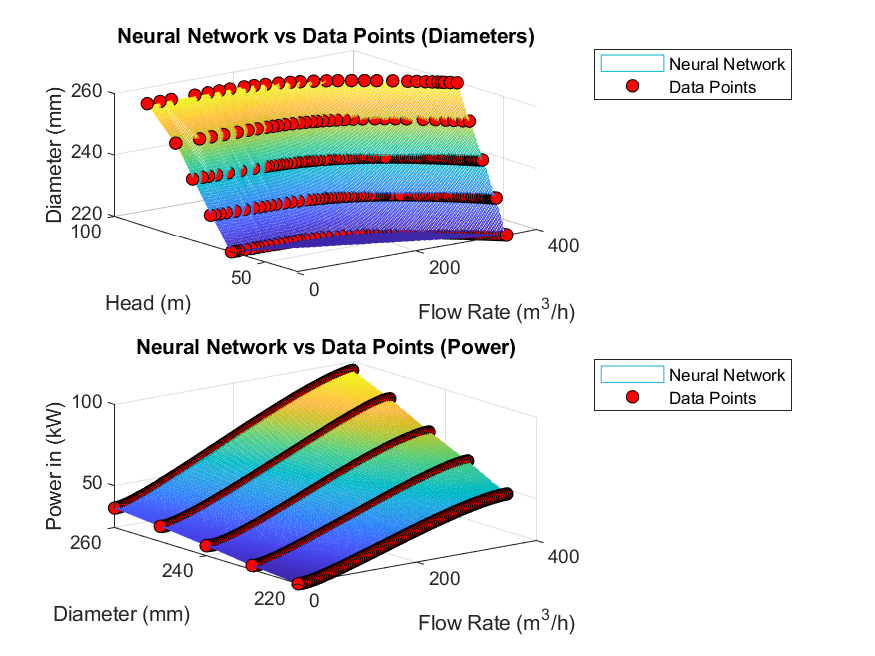
\includegraphics{diameter_power_visualization_2024-04-30_18-58-24.png}

}

\caption{\label{fig-NNvsData}NN vs Data}

\end{figure}%


  \bibliography{references.bib}


\nocite{*}

\end{document}
